\section{Text Representation in Legal Judgments}


\subsection{Corpus Processing}

% Warning!! Copy/Paste
% Pré-processamento
After text extraction from the documents, we applied some pre-processing steps, which are required before training the embeddings or text classification. The first of them was the conversion to lower case. Then punctuation marks were removed, as well as special characters and some symbol characters. We removed stopwords neither apply stemmization or lemmatization, following the literature  \cite{Mikolov2013, Pennington2014}.

% Warning!! Copy/Paste
% Sobre a divisão da base maior em bases de tamanho menor
In relation to our three corpora used in embeddings training, which comprising 3.7 billion, 100 million  and 1.19 bilion words for \emph{general}, \emph{air transport} and \emph{global} corpora, respectively, we created others based on them according to the following smaller corpora sizes, considering the word count: 1,000; 10,000; 50,000; 100,000; 200,000; 500,000; 1,000,000; 5,000,000; 10,000,000; 25,000,000; 100,000,000; 500,000,000; 750,000,000 and 1,000,000,000.

% Warning!! Copy/Paste
% Porque dividimos nesses tamanhos de base.
We choose these corpora sizes to be able to compare the variation on evaluation metrics while increasing corpora size. For the air transport context, we could not embrace all these sizes due to limited corpora available. The largest sub-base had  100 million words for this context. 

% Warning!! Copy/Paste
% Cada uma dessas bases vai ser usada pra treinar um embedding diferente.
Finally, each of these smaller corpora was used to train one different word embeddings representation.

\subsection{Embeddings Training}

% Warning!! Copy/Paste
% Usamos esse algoritmo pois tem dado bons resultados e também pelo tempo de treinamento ser bem menor
In this work, we chose GloVe representation due to its good results in many NLP tasks, including text classification, and also for its training time which is significantly less than other techniques like Word2Vec and FastText \cite{Pennington2014}.  
% Parâmetros do algoritmo
In terms of GloVe parameters, we kept most of the default values, except for windows size, training iterations, and vector size, which were set to 5, 100, and 100, respectively. With these values, we achieved better results in text classification.

% Warning!! Copy/Paste
Considering the corpus sizes described in Section \ref{sec:corpus_construction} and the parameters above described, we trained 15 representations for \emph{general} and \emph{global} contexts bases. For \textit{air transport} context base, we trained 11 embeddings.

\subsection{Embeddings Evaluation in Legal Text Classification}

% Warning!! Copy/Paste
To evaluate the GloVe embeddings representations, we applied each of them to the task of text classification on judgments from JEC/UFSC. Also, we used Convolutional Neural Networks as a classification model based on the literature \cite{Kim2014}. Fig. \ref{fig:cnn_model} illustrates this model.

% Demonstrar um gráfico com a CNN.
\begin{figure}[htb]
    \centering
    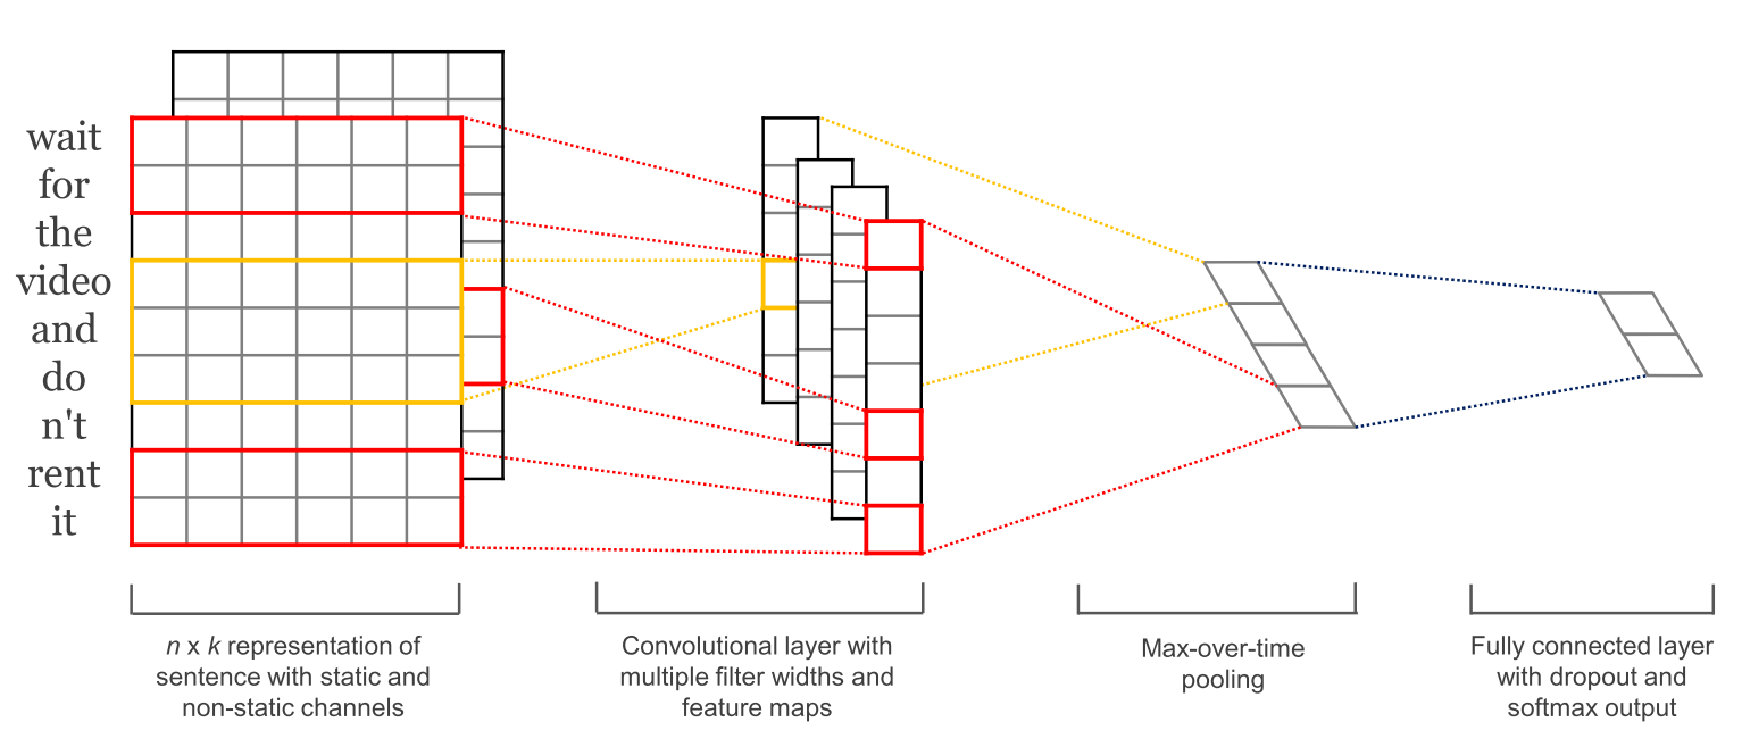
\includegraphics[width=\textwidth]{images/cnn_model.pdf}
    \caption{CNN Model for Text Classification \cite{Kim2014}}
    \label{fig:cnn_model}
\end{figure}

% Warning!! Copy/Paste
% A CNN mostrada leva em conta a ordem das palavras
This CNN takes into account the order of the words by stacking the corresponding embeddings for each word as they occur in the text. 
% São aplicados filtros de convolução com diversas dimensão, onde a largura corresponde ao tamanho dos embeddings e a altura o número de embeddings que serão englobados pelo filtro.
% Warning!! Copy/Paste
Them it applies multiple convolutional masks with different dimensions that correspond to the red and yellow contours in Fig. \ref{fig:cnn_model}. Mask widths are equal to word embedding size while the heights can vary. In this context, mask height can be related to the idea of N-Grams, since they embrace multiple embeddings at the same time. 
% No original tinha 3 tamanhos de filtro, mas incluímos um mais que melhorou os resultados. Em número de filtros, tinha 100 e abaixamos pra 10 sem piorar o desempenho, mas tornando
% Warning!! Copy/Paste
In the original model, these heights were set to 3, 4, and 5. We added one more mask of height 2, which increased classification metrics. Also, we set to 10 the number of masks for each of these sizes, without affecting our results, but decreasing the required training time. 

% Warning!! Copy/Paste
% Explicar sobre como esse modelo foi utilizado
In this work, we applied each of the embeddings trained in conjunction with the CNN described in the classification of JEC/UFSC judgments, where Out of Vocabulary (OOV) words are replaced by an vector of random values. Thus, we trained and tested 41 models. Furthermore, due to the stochastic nature of neural networks training methods \cite{Cohen1995}, each of these models was trained and tested 200 times and the resulting evaluation metrics were averaged. 

% Warning!! Copy/Paste
Finally, we compare the performance in classification using Accuracy and Macro F1-Score.


% \subsection{Results Analysis and Discussion}

% % Warning!! Copy/Paste
% In the following sections, we present and discuss our results for text classification using trained embeddings for \emph{global}, \emph{general}, and \emph{air transport} contexts with multiple corpus training sizes. %Then, these results are discussed from contexts and corpus size perspectives.

% Warning!! Copy/Paste
% Experimental results
\subsection{Experimental Results}

% Warning!! Copy/Paste
Following the steps presented in section~\ref{sec:experiments}, we trained all 41 word embeddings representations for GloVe. 

% Warning!! Copy/Paste
To illustrate how these embeddings behave, in Fig.~\ref{fig:projection}, we used Principal Component Analysis (PCA) to create a projection in two dimensions of a set of words from \textit{general} context embedding trained with 1 billion words.

\begin{figure}[htb]
    \centering
    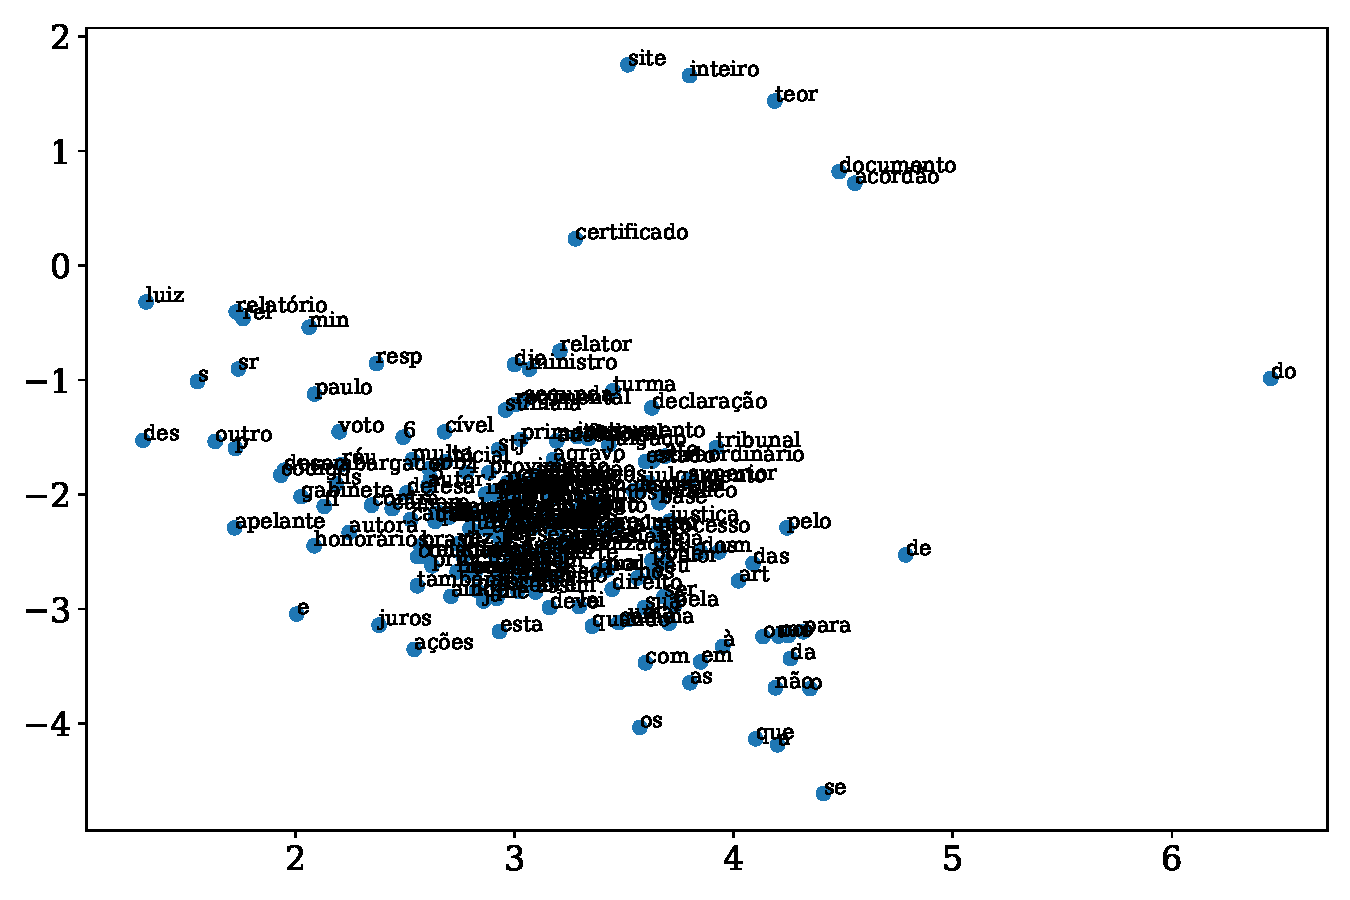
\includegraphics[width=0.9\textwidth]{images/projection.pdf}
    \caption{Word Embeddings Projection}
    \label{fig:projection}
\end{figure}

% Warning!! Copy/Paste
%%%% FIGURE- Embeddings projection
Using each embedding, we trained and tested CNNs for text classification in JEC/UFSC judgments. These two steps were repeated 200 times, and the evaluation metrics were averaged for each group of repetitions.

% Warning!! Copy/Paste
In Fig. \ref{fig:accuracy_plot} and \ref{fig:f1_plot}, we present the results, for accuracy and F1-Score, respectively, from test data applied to each CNN model. These results are related to embeddings trained with \textit{general}, \textit{air transport}, \textit{global} texts. 
The x-axis denotes the corpus sizes used to train the embeddings, while the y-axis represents accuracy or F1-Score. Each data point represents the average of the evaluation metric, after 200 train and test repetitions using each specific embedding. %Finally, we delimited y-axis to smaller intervals so the metrics variations could be visible.


% JH In the next section, we discuss these results.

\begin{figure}[htb]
    \centering
    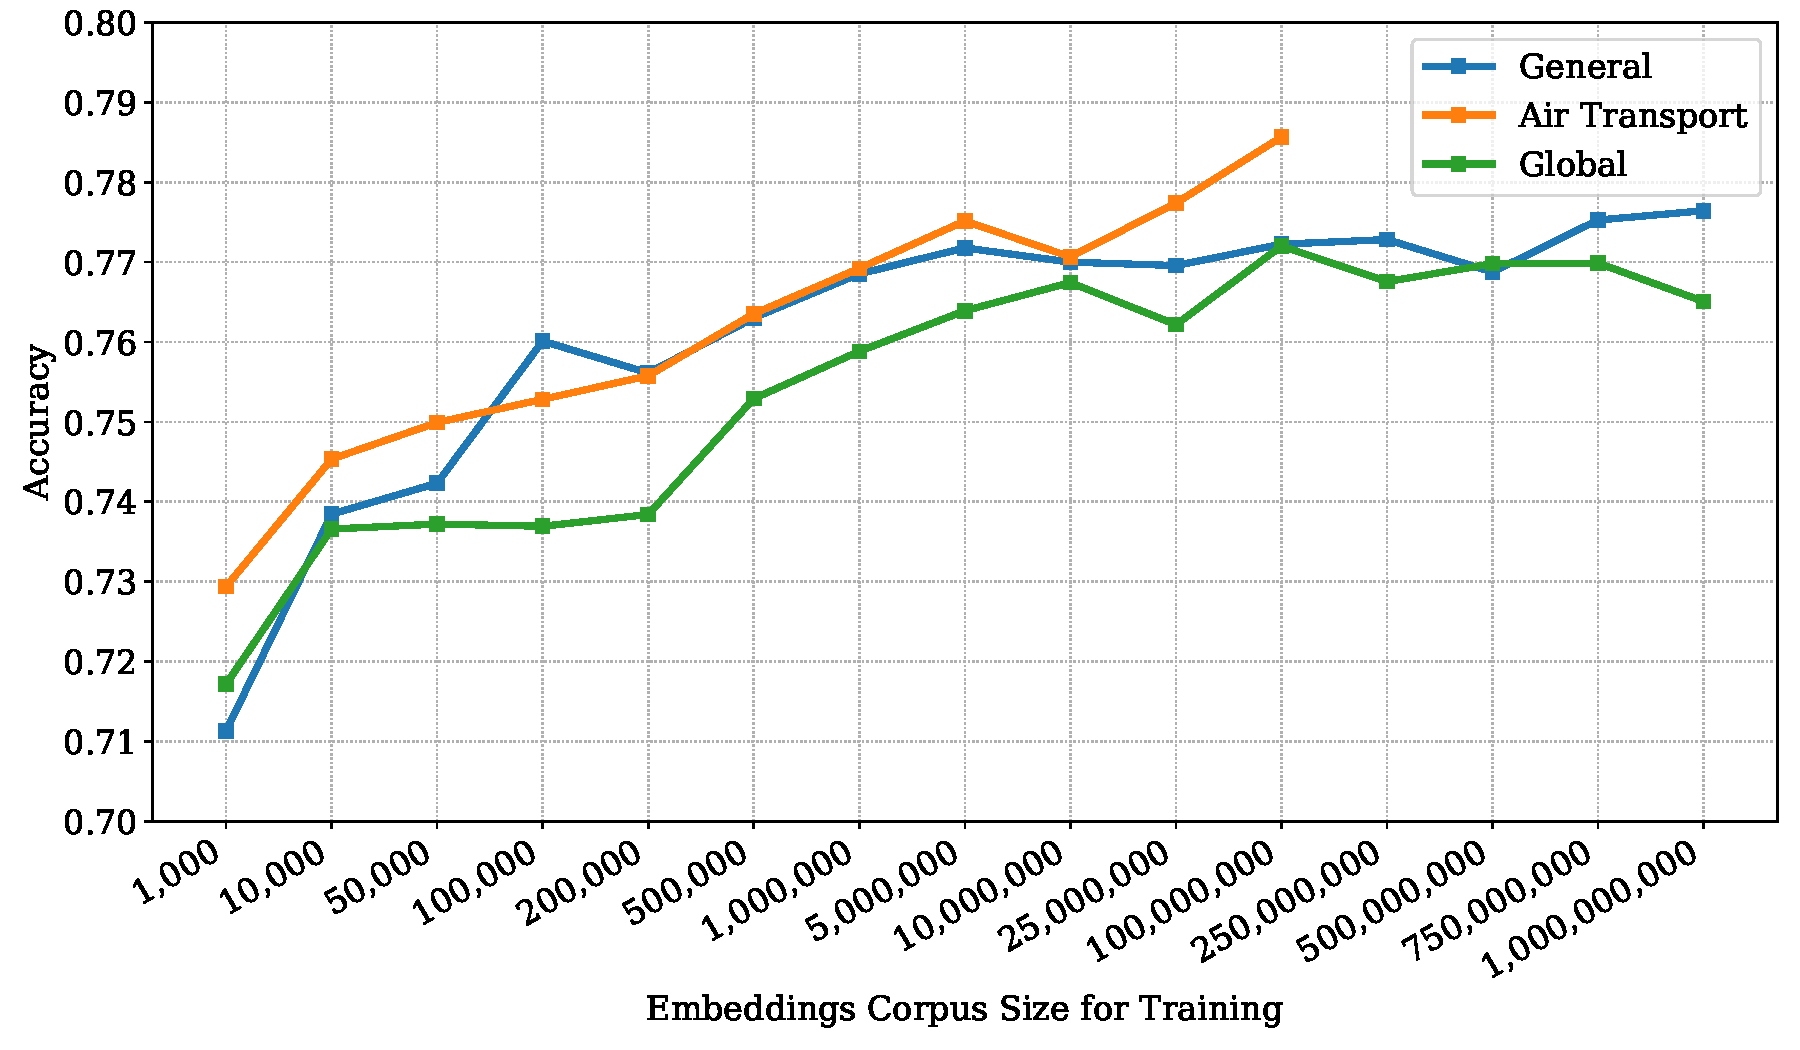
\includegraphics[width=0.9\textwidth]{images/acc_mean_final.pdf}
    \caption{Accuracy for test set from CNN model}
    \label{fig:accuracy_plot}
\end{figure}

\begin{figure}[htb]
    \centering
    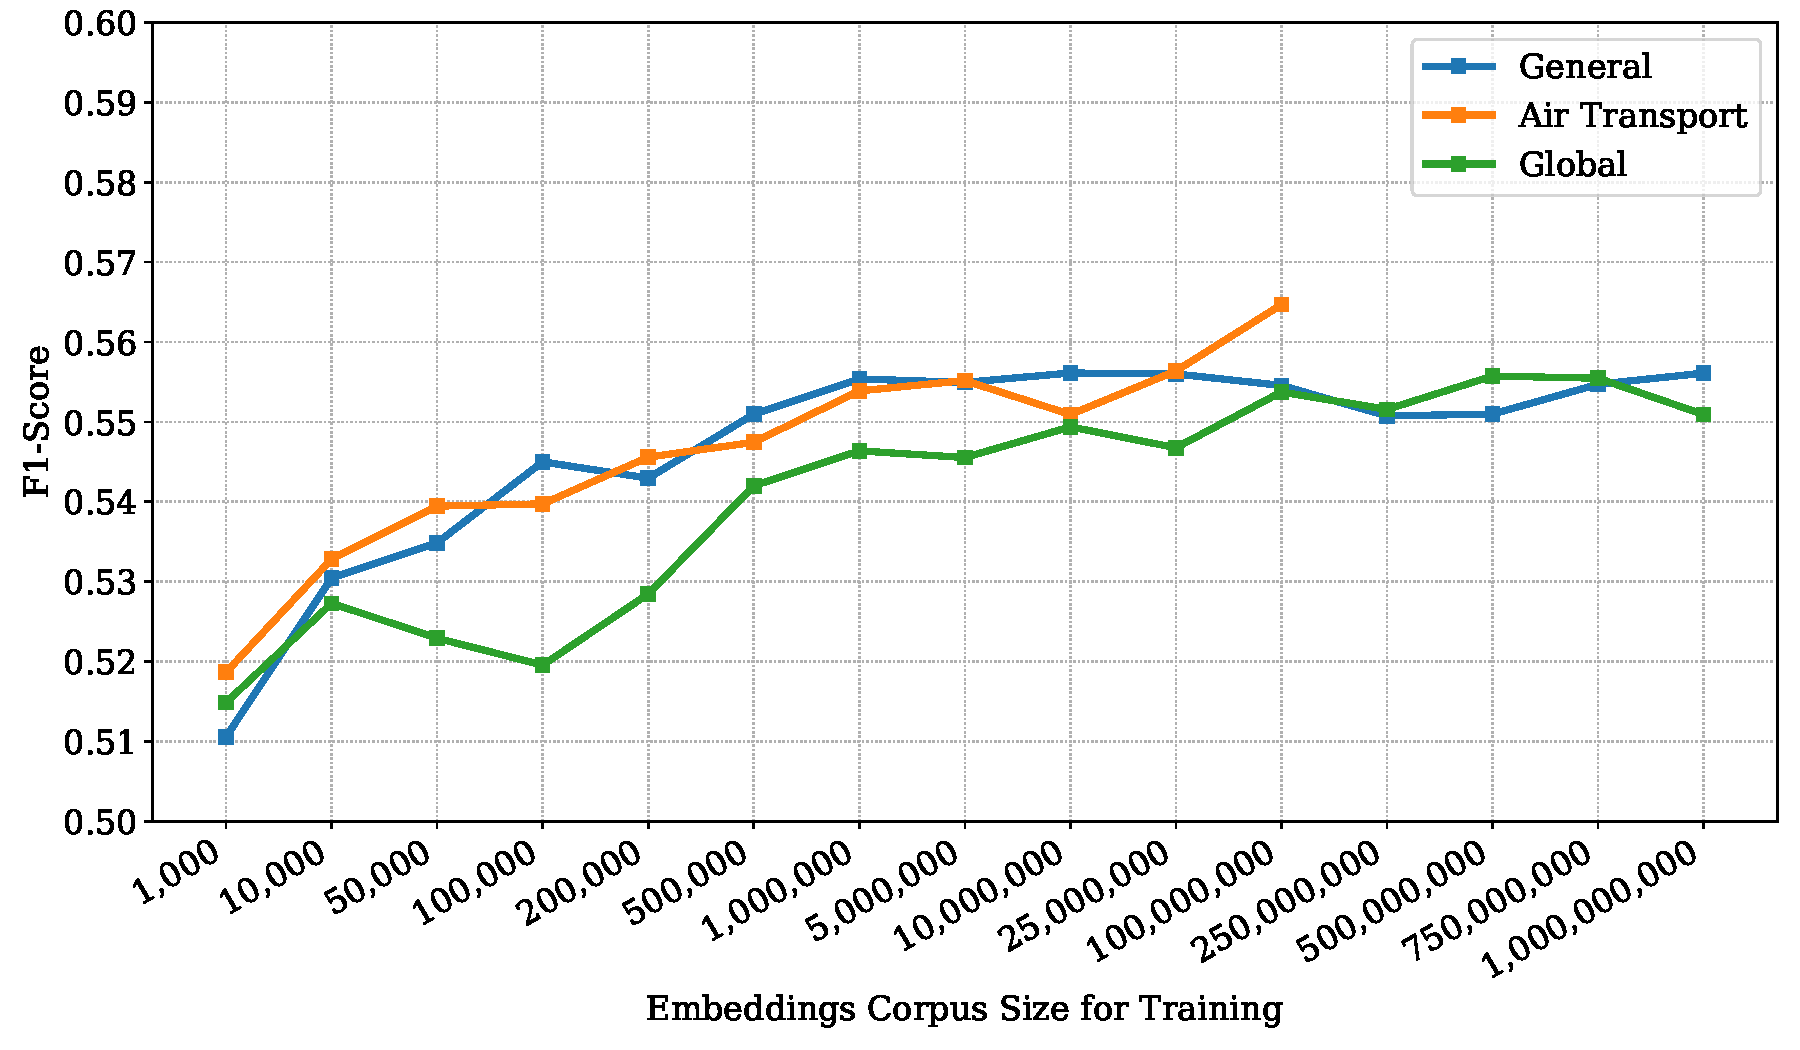
\includegraphics[width=0.9\textwidth]{images/f1_score_mean_final.pdf}
    \caption{Macro F1-Score for test set from CNN model}
    \label{fig:f1_plot}
\end{figure}

% Evaluations from context perspective
\subsection{Discussion from Context Perspective}

% Warning!! Copy/Paste
In this section, we will consider the first part of our research question: Does the specificity of the corpora in embeddings training contribute to the quality of the classification? 

% Warning!! Copy/Paste
In terms of accuracy, when we compare \emph{global} against others (Fig.~\ref{fig:accuracy_plot}), we have that higher text specificity leads to better results, for most of the corpus sizes used for embeddings training. Furthermore, when comparing \textit{general} and \textit{air transport} curves, there is a significant difference in accuracy only for the lowest and highest x-values. 
However, in terms of F1-Score, as shown in Fig. \ref{fig:f1_plot}, our observations change, once \textit{general} and \textit{air transport} curves have a similar shape. Also, for the highest corpus sizes, \textit{general} and \textit{global} curves converge to similar values of F1-Score. 
%
% Warning!! Copy/Paste
We believe that these differences in accuracy and F1-Score emerge from the fact that our dataset to text classification is imbalanced, once the former does not take this fact into account, while the latter does. However, this result still requires further investigation. 
% Warning!! Copy/Paste
In general, we can note that for smaller corpora size for embeddings training, text specificity has a more impact than for large sizes.


% Evaluation from corpus size perspective
\subsection{Discussion from Corpus Size Perspective}

% Warning!! Copy/Paste
In this section, we will consider the second part of our research question: How does the corpus size contribute to the embedding quality?

% Warning!! Copy/Paste
When we observe both accuracy and F1-Score measures from Fig.~\ref{fig:accuracy_plot} and \ref{fig:f1_plot}, it is clear the tendency for improvement while increasing corpus size. However, the metrics converge with the largest corpus sizes. There are two exceptions. The first one occurs with smaller values of corpus sizes for \textit{global} curve, as it decreases in F1-Score measures. The second corresponds to the last data point in \textit{air transport} curves. The former can happen we the classifier performs poorly for some classes while gets better in others. The latter may indicate that those curves could improve if we had more significant corpus sizes related to that context.

% Warning!! Copy/Paste
In general, we can note that the greater the corpus size in embeddings training, the better are the results. However, this impact decreases as the corpus size increases until a point where more words in the corpus have little impact on the results. %On the other hand, in the smaller corpus, the impact of increasing them is higher in relation to the greater corpus.